%\chapterimage{Geometrijska.jpg} % Chapter heading image

\chapter{Optika v anizotropnih snoveh}
\label{chap:AnizotropneSnovi}
V tem poglavju bomo spoznali optično anizotropne snovi, katerih odziv na 
vpadno svetlobo je odvisen od njene polarizacije. Opisali bomo 
širjenje svetlobe skozi anizotropne snovi in pojasnili razliko med optično 
enoosnimi in optično dvoosnimi snovmi. Spoznali bomo dvojni lom in 
na koncu poglavja predstavili nekaj načinov uporabe tega zanimivega pojava.

\section{Anizotropne snovi}
Do zdaj smo obravnavali izotropne snovi, v katerih je lomni količnik 
snovi enak v vseh smereh in za vse polarizacije vpadne svetlobe. 
Za anizotropne snovi pa je značilno, da imajo 
v različnih smereh različne lastnosti, na primer mehanske, toplotne, 
električne, magnetne, optične ... Primeri optično 
anizotropnih snovi so kremen, kalcit, led, sljuda, tekoči kristali
in tudi raztegnjeni polimerni vzorci, na primer celofan ali prozorni lepilni trak. 
Optično anizotropne snovi najlaže prepoznamo po barvitih vzorcih med
polarizatorjema, ki spreminjajo barvo, ko polarizatorja sučemo. 
Zakaj je tako, bomo spoznali v nadaljevanju poglavja.
\begin{figure}[ht]
\centering
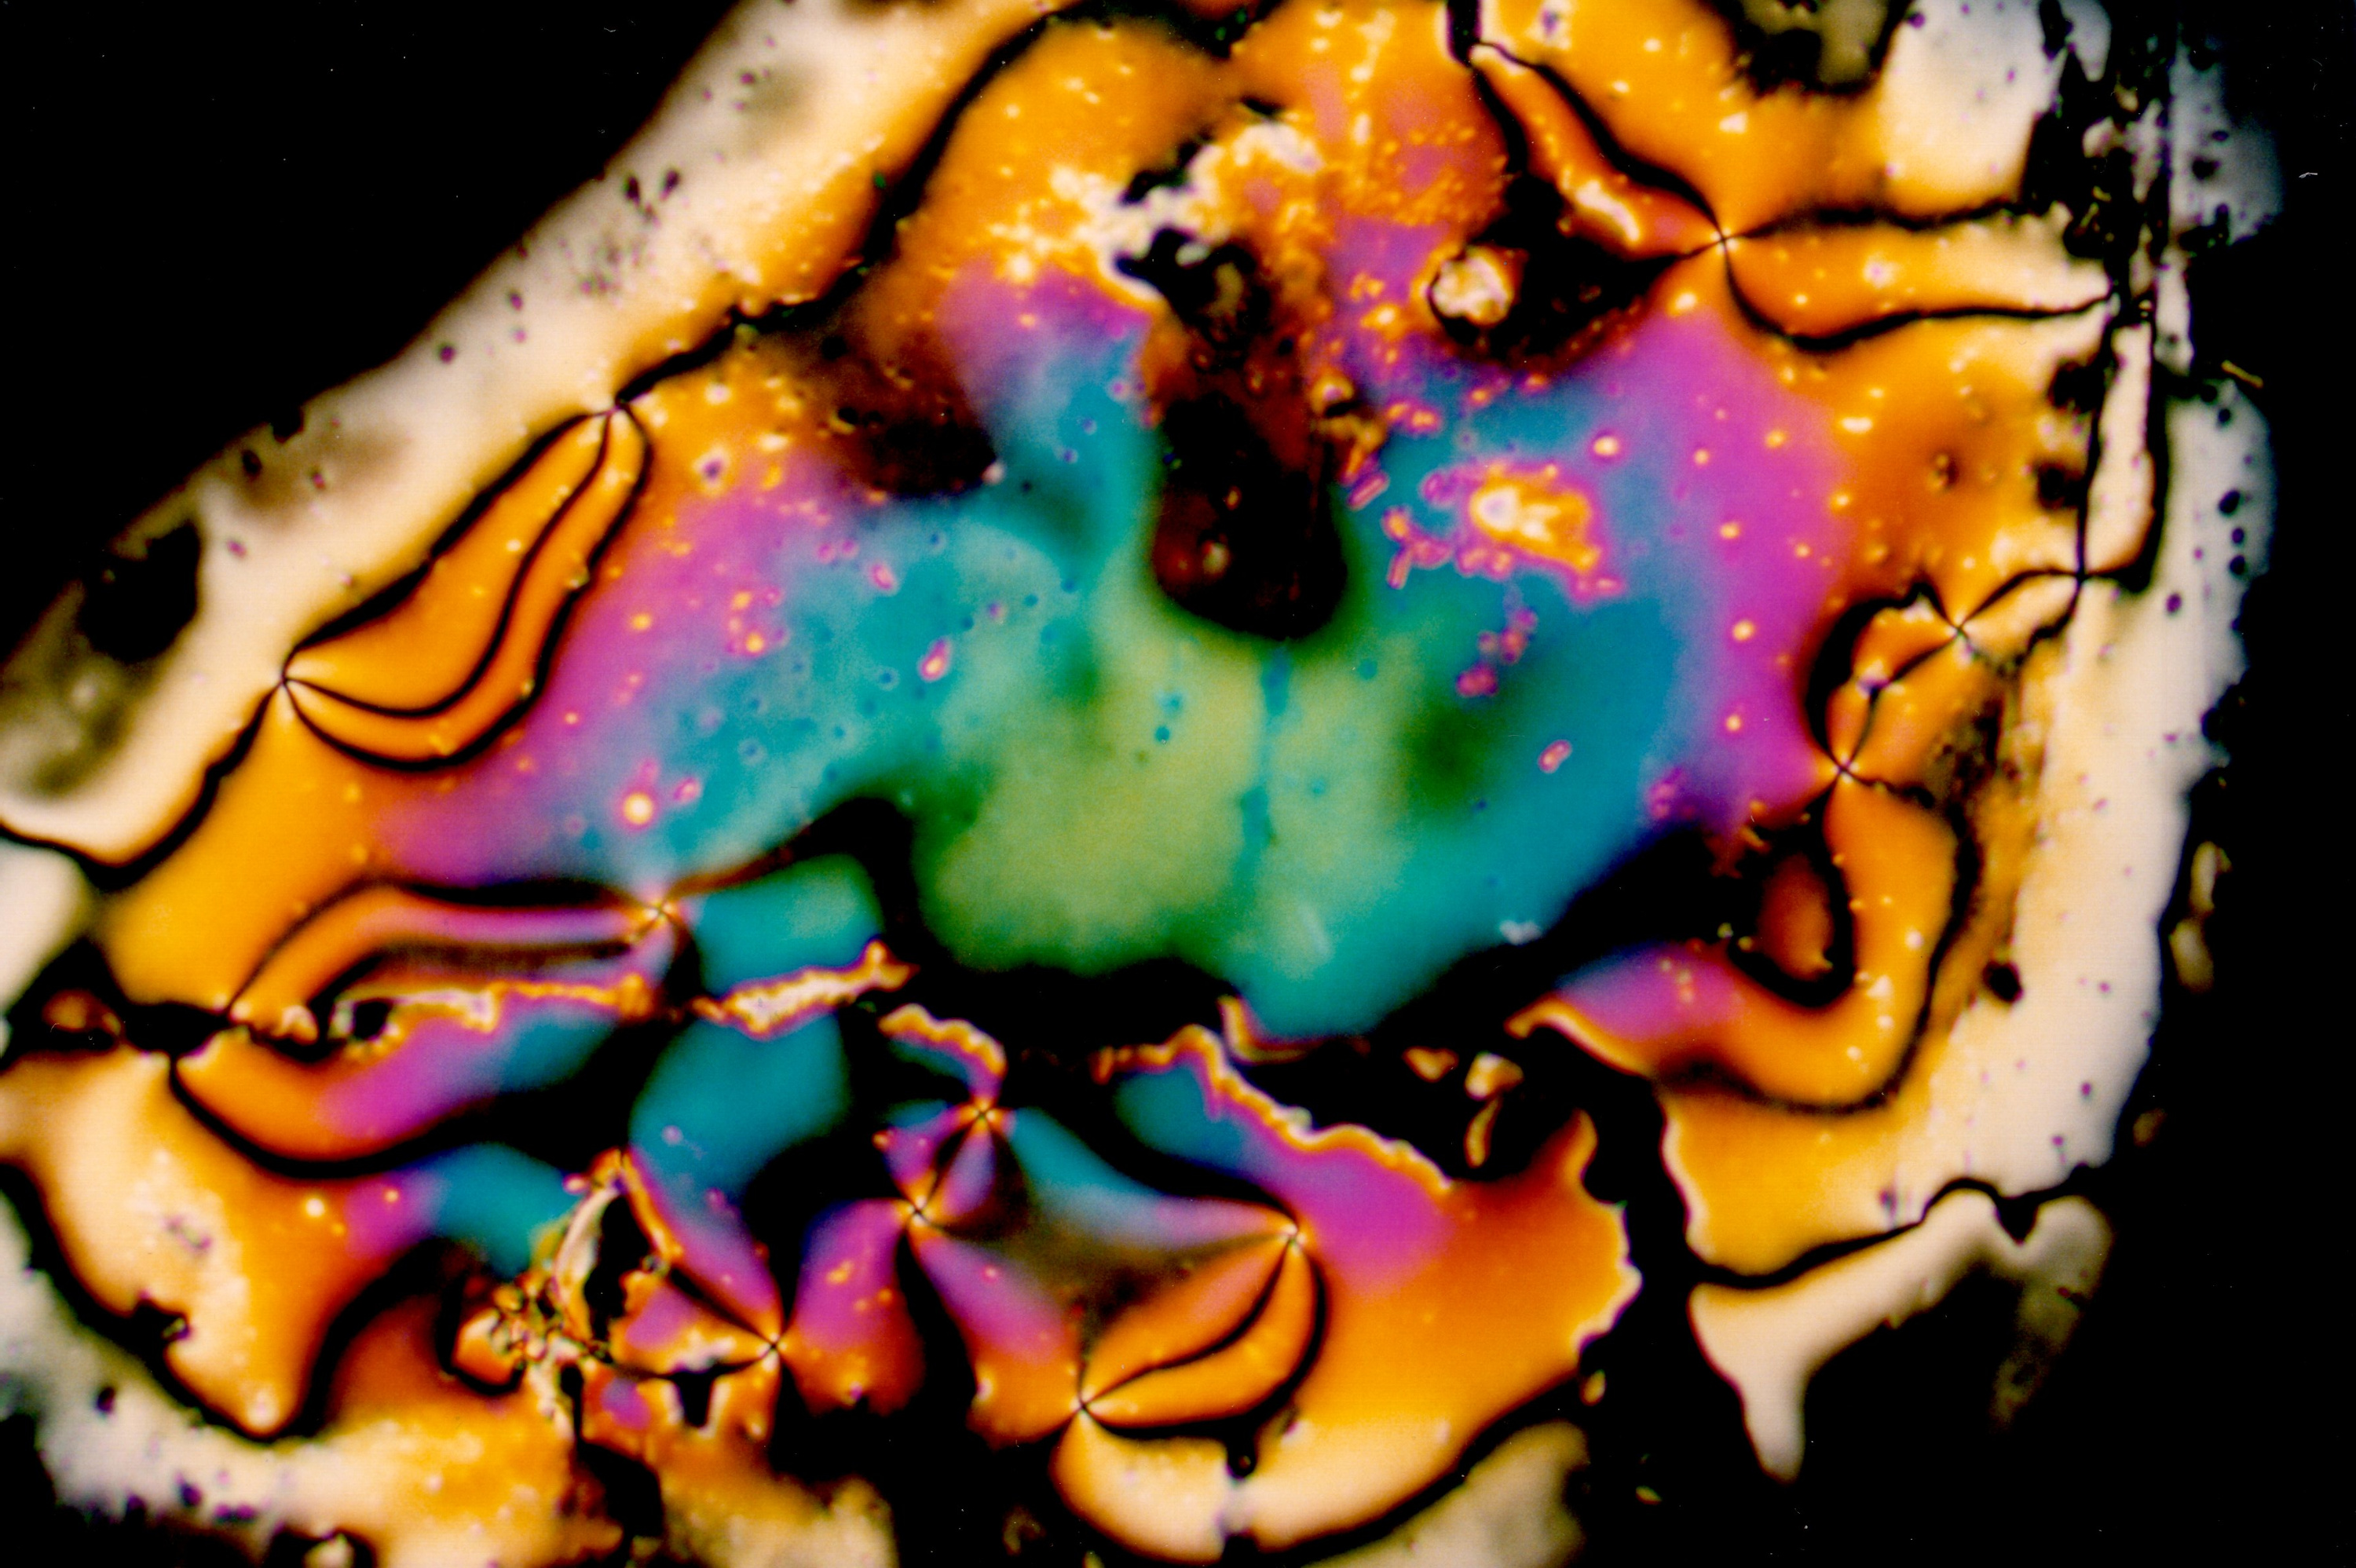
\includegraphics[width=7truecm]{slike/10_foto_nematik.jpg}\hfill
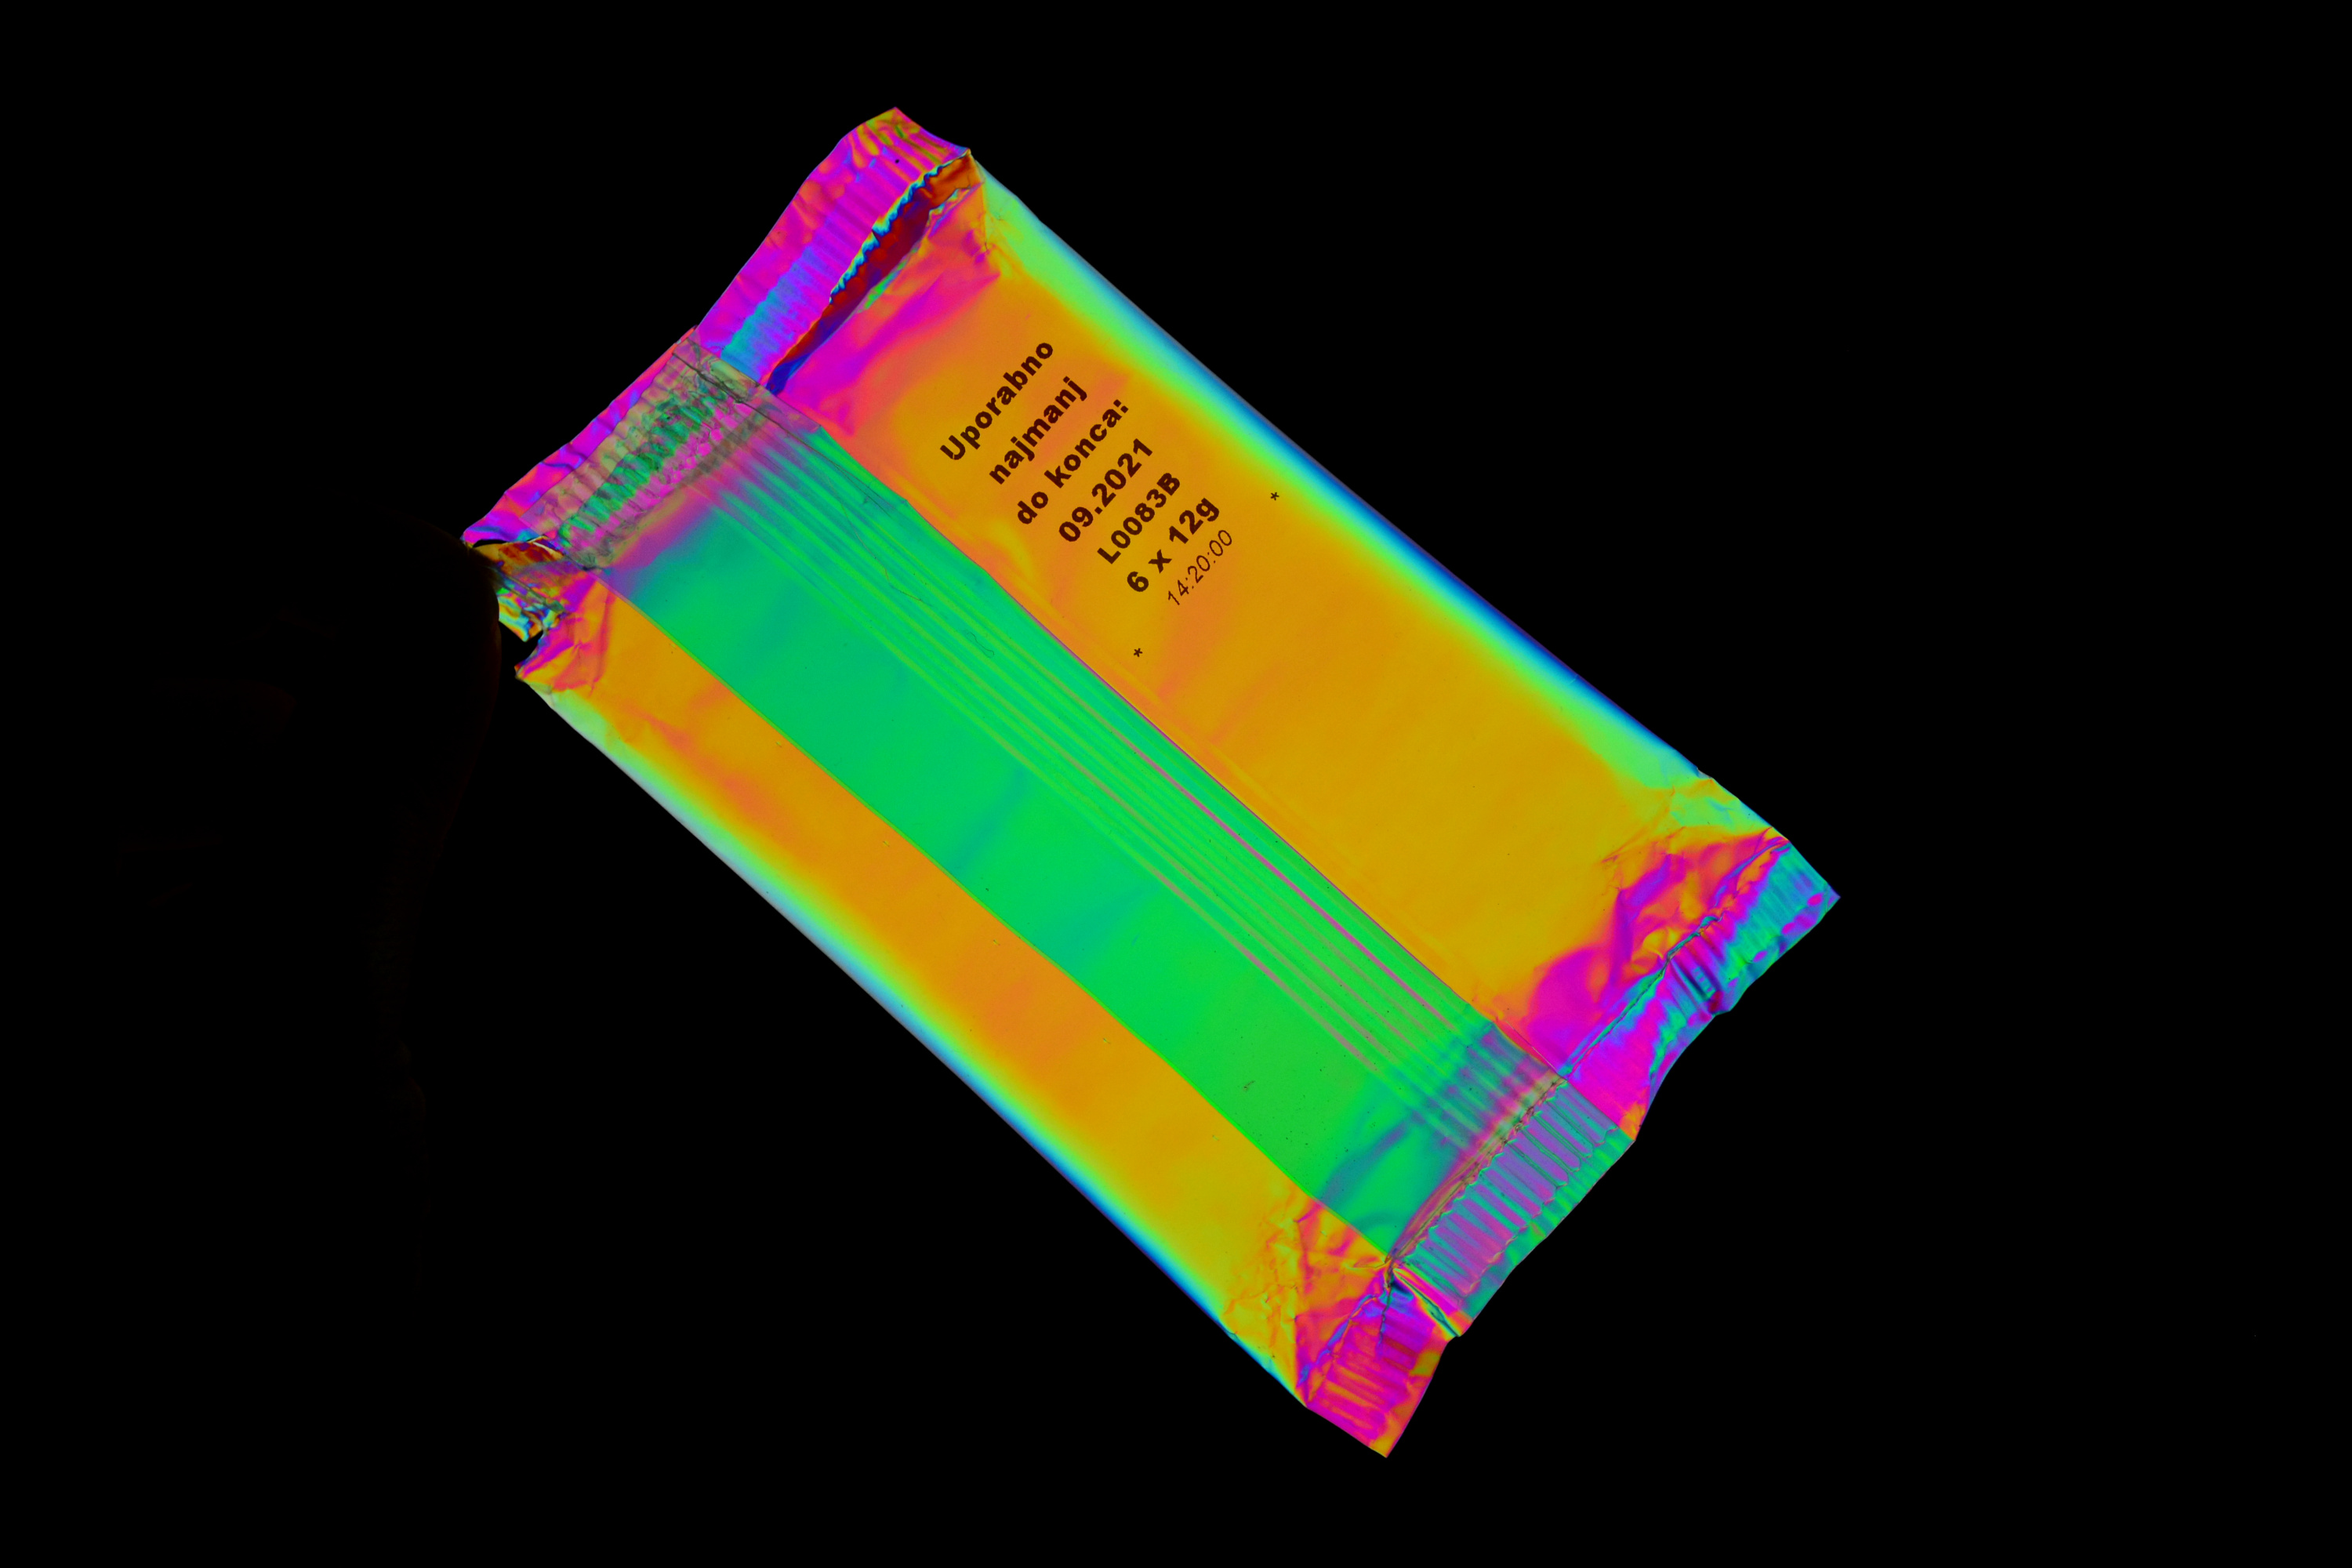
\includegraphics[width=7truecm]{slike/10_foto_celofan.jpg}
\caption{Kapljica tekočega kristala, ki je anizotropna tekočina, slikana pod 
mikroskopom (levo) in ovitek iz celofana (desno). Oba vzorca sta bila postavljena
med prekrižana polarizatorja.}
\label{fig:10_nematik}
\end{figure}

Najznačilnejša optična lastnost anizotropnih snovi je odvisnost lomnega
količnika od smeri širjenja svetlobe in njene polarizacije. Pojav
je posledica odziva snovi na vpadno svetlobo, pri katerem smer in 
velikost inducirane električne polarizacije določa struktura snovi.  
Za nazorno razlago se ponovno poslužimo
Lorentzevega modela, ki smo ga podrobneje spoznali v prejšnjem 
poglavju (glej razdelek~\ref{chap:lomni}). 

Zamislimo si negativno nabito kroglico, ki predstavlja elektron, vpeto v 
mrežo mirujočih sosednjih kroglic, ki predstavljajo pozitivne ione kristala. 
Vzmeti, ki kroglice medsebojno povezujejo, niso vse enake, ampak imajo različne 
konstante vzmeti, odvisno od smeri (slika~\ref{fig:10_model}\,a). Ko na elektron
vpade svetloba, ga sila električnega polja izmakne iz ravnovesne lege, tej sili 
pa nasprotujejo sile vzmeti. Premik elektrona je večji v smeri šibkejše vzmeti, 
zato dipolni moment, ki ga povzroči premik elektrona, ni vzporeden jakosti 
vpadnega električnega
polja. 
\begin{figure}[!h]
\centering
\def\svgwidth{120truemm} 
\input{slike/10_Lorentz_a.pdf_tex}
\caption{Anizotropijo snovi lahko pojasnimo z Lorenzevim modelom, v katerem so
konstante vzmeti, s katerimi je v snov vezan elektron, različne  in $k_1 \neq k_2 \neq k_3$ (a).
V anizotropnih snoveh inducirana električna polarizacija $\mathbf{P}$ ni vzporedna 
z jakosto električnega polja $\mathbf{E}$ (b).}
\label{fig:10_model}
\end{figure}

Osnovna posledica anizotropnega odziva je, da smer inducirane električne polarizacije $\mathbf{P}$
 v anizotropnih snoveh ni vzporedna smeri jakosti optičnega električnega polja $\mathbf{E}$ 
(slika~\ref{fig:10_model}\,b). Posledično tudi 
vektor gostote električnega polja $\mathbf{D}$ ni vzporeden s smerjo $\mathbf{E}$. 
Linearni odziv snovi zapišemo kot:
\beq
\mathbf{D} = \varepsilon_0 \mathbf{E} + \mathbf{P} = \varepsilon_0 \underline{\varepsilon} \mathbf{E}.
\label{eq:10_001}
\eeq
Vpeljali smo tenzor dielektričnosti $\underline{\varepsilon}$, ki je v anizotropnih snoveh na splošno 
tenzor drugega ranga:
\beq
\underline{\varepsilon} = 
\left[\begin{array}{ccc}
\varepsilon_{xx} & \varepsilon_{xy} & \varepsilon_{xz}\\
\varepsilon_{yx} & \varepsilon_{yy} & \varepsilon_{yz}\\
\varepsilon_{zx} & \varepsilon_{zy} & \varepsilon_{zz}\\
\end{array}\right]\!\!.
\label{eq:10_002}
\eeq
\begin{remark}
Pri obravnavi se bomo omejili na prozorne optično neaktivne anizotropne snovi. 
Ker dielektričnost nastopa v izrazu za energijo elektromagnetnega polja 
(enačba~\ref{eq:03_27}), je zaradi ohranitve energije tenzor $\underline{\varepsilon}$ na splošno
Hermitski in pozitivno definiten. V našem primeru to pomeni, da je 
tenzor simetričen in ga lahko vedno diagonaliziramo, pri čemer so 
vse njegove lastne vrednosti realne in pozitivne.
\end{remark}

Tenzor dielektričnosti diagonaliziramo in v lastnem koordinatnem 
sistemu ga zapišemo kot:
\beq
\underline{\varepsilon} = 
\left[\begin{array}{ccc}
\varepsilon_{xx} & 0 & 0\\
0 & \varepsilon_{yy} &0\\
0 & 0 & \varepsilon_{zz}\\
\end{array}\right]\!\!.
\label{eq:10_003}
\eeq
Po dogovoru koordinatni sistem navadno izberemo tako, da velja 
$\varepsilon_{xx}<\varepsilon_{yy}<\varepsilon_{zz}$.

Na splošno so vse tri neničelne komponente diagonalnega tenzorja različne. 
Pri snoveh z večjo stopnjo simetrije sta dve komponenti enaki ($\varepsilon_{xx} = 
\varepsilon_{yy} \neq \varepsilon_{zz}$), v izotropnih snoveh pa so vse tri 
neničelne komponente tenzorja enake. 

\begin{example}{\bf Smeri jakosti električnega polja 
in inducirane polarizacije v anizotropni snovi.}
Naj na anizotropno snov vpada elektromagnetno valovanje vzdolž osi $z$. Jakost
električnega polja na splošno leži v ravnini $xy$ in naj z osjo $x$ oklepa kot $\alpha$. 
Po komponentah jo zapišemo kot $\mathbf{E} = (E_x, E_y, 0)$. 

Iz enačbe~(\ref{eq:10_001}) sledi zveza:
\beq
\mathbf{P} = \varepsilon_0 \left(\underline{\varepsilon} - \underline{I}\right)\mathbf{E}
\label{eq:10_004}
\eeq
Vstavimo vektor $\mathbf{E}$ in v lastnem koordinatnem sistemu tenzorja 
dielektričnosti (enačba~\ref{eq:10_003}) inducirano električno polarizacijo zapišemo kot:
\begin{align}
P_x &= (\varepsilon_{xx}-1) \varepsilon_0 E_x \qquad \mathrm{in} \label{eq:10_005}\\
P_y &= (\varepsilon_{yy}-1) \varepsilon_0 E_y.
\label{eq:10_006}
\end{align}
Kot $\beta$, ki ga inducirana električna polarizacija oklepa z osjo $x$, izračunamo iz enačbe:
\beq
\tan \beta = \frac{P_y}{P_x} = \frac{(\varepsilon_{yy}-1)E_y}{(\varepsilon_{xx}-1)E_x}
 = \frac{\varepsilon_{yy}-1}{\varepsilon_{xx}-1}\tan \alpha.
\eeq
\end{example}

\section{Ravni val v anizotropni snovi}
Poglejmo najprej, kako se po optično anizotropni snovi širi ravni val. 
Obravnavajmo optično anizotropno neprevodno snov, katere dielektričnost 
opišemo s tenzorjem $\underline{\varepsilon}$ (enačba~\ref{eq:10_003}). 
Zaradi enostavnosti se omejimo na nemagnetne snovi, za katere je $\mu = 1$. 
Naj na tako snov vpada ravno potujoče sinusno valovanje z 
valovnim vektorjem $\mathbf{k}$.  

Za opis valovanja izhajamo iz Maxwellovih enačb (enačbe~\ref{eq:Maxwell1}--\ref{eq:Maxwell4}), 
pri čemer privzamemo, da sta gostoti nabojev in električnih tokov enaki nič. 
Rešitev iščemo v obliki ravnih valov:
\begin{align}
 \mathbf{E} &= \mathbf{E}_0 e^{i\mathbf{k}\cdot \mathbf{r} - i \omega t} \label{eq:10_010} \\
 \mathbf{D} &= \mathbf{D}_0 e^{i\mathbf{k}\cdot \mathbf{r} - i \omega t} \label{eq:10_011}\\
 \mathbf{B} &= \mu_0 \mathbf{H} = \mathbf{B}_0 e^{i\mathbf{k}\cdot \mathbf{r} - i \omega t}.
 \label{eq:10_012}
\end{align}
Iz Maxwellove enačbe~(\ref{eq:Maxwell3}) dobimo z upoštevanjem nastavkov:
\beq
\nabla \cdot \left(\mathbf{D}_0 e^{i\mathbf{k}\cdot \mathbf{r} - i \omega t} \right) = 
i\,\mathbf{k}\cdot \mathbf{D} = 0 \qquad \Longrightarrow \qquad \mathbf{D} \perp \mathbf{k}.
\label{eq:10_013}
\eeq
Podobno iz enačbe~(\ref{eq:Maxwell4}) sledi:
\beq
\nabla \cdot \left(\mathbf{B}_0 e^{i\mathbf{k}\cdot \mathbf{r} - i \omega t} \right) = 
i\,\mathbf{k}\cdot \mathbf{B} = 0 \qquad \Longrightarrow \qquad \mathbf{B} \perp \mathbf{k}.
\label{eq:10_014}
\eeq
Povsem na splošno sta torej vektorja $\mathbf{D}$ in $\mathbf{B}$ pravokotna na valovni vektor $\mathbf{k}$.
Izhajajoč iz enačbe~(\ref{eq:Maxwell1}) dobimo:
\beq
\nabla \times \left(\mathbf{H}_0 e^{i\mathbf{k}\cdot \mathbf{r} - i \omega t} \right) = 
i\,\mathbf{k}\times \mathbf{H} = \frac{\partial \mathbf{D}}{\partial t} = -i \omega \mathbf{D}.
\label{eq:10_015}
\eeq
Od tod za nemagnetne snovi neposredno sledi:
\beq
\mathbf{k}\times \mathbf{B} = - \mu_0 \omega \mathbf{D} \qquad \Longrightarrow \qquad \mathbf{B} \perp \mathbf{D}.
\label{eq:10_016}
\eeq
Vektorji $\mathbf{D}$, $\mathbf{B}$ in $\mathbf{k}$ so torej medsebojno paroma pravokotni.

Uporabimo nastavke (enačbe~\ref{eq:10_010}--\ref{eq:10_012})
še v Faradayevem zakonu (enačbo~\ref{eq:Maxwell2}) in dobimo:
\beq
\nabla \times \left(\mathbf{E}_0 e^{i\mathbf{k}\cdot \mathbf{r} - i \omega t} \right) = 
i\,\mathbf{k}\times \mathbf{E} = - \frac{\partial \mathbf{B}}{\partial t} = i \omega \mathbf{B}.
\label{eq:10_017}
\eeq
Dobimo:
\beq
\mathbf{k}\times \mathbf{E} = \omega \mu_0 \mathbf{H} \qquad \Longrightarrow 
\qquad \mathbf{E} \perp \mathbf{H}.
\label{eq:10_018}
\eeq
Upoštevamo še definicijo Poyntinovega vektorja 
(enačba~\ref{eq:Poyntingov}) $\mathbf{S} = \mathbf{E} \times \mathbf{H}$, od koder
sledi medsebojna pravokotnost vektorjev $\mathbf{E}$, $\mathbf{H}$ in $\mathbf{S}$.

Ker v anizotropnih snoveh vektorja jakosti in gostote električnega 
polja nista vzporedna, tudi valovni vektor in Poyntingov vektor nista 
vzporedna. Energija, ki potuje v smeri Poyntingovega vektorja, se
torej v anizotropnih snoveh ne širi vzdolž valovnega vektorja (slika~\ref{fig:10_koti}). 
\begin{figure}[!h]
\centering
\def\svgwidth{40truemm} 
\input{slike/10_koti_Sk.pdf_tex}
\caption{V anizotropnih snoveh smer Poyntingovega 
vektorja $\mathbf{S}$ ni enaka smeri valovnega vektorja $\mathbf{k}$.}
\label{fig:10_koti}
\end{figure}

V anizotropnih snoveh elektromagnetno valovanje ostaja transverzalno
valovanje le s stališča vektorjev $\mathbf{D}$, $\mathbf{B}$ in 
$\mathbf{k}$. Električna poljska jakost $\mathbf{E}$ pa pridobi 
tudi longitudinalno komponento vzdolž smeri valovnega vektorja. 
Zveza $\nabla \cdot \mathbf{D} = 0$ zato še vedno velja, zveza 
$\nabla \cdot \mathbf{E} = 0$ pa ne več. Posledično tudi valovna
enačba za jakost električnega polja, kakor smo je vajeni
v izotropnih snoveh, v anizotropnih snoveh ne velja. Zapišimo 
analogno enačbo za anizotropne snovi. 

Izhajamo iz Maxwellove enačbe (\ref{eq:Maxwell2}) in na njej naredimo rotor:
\beq
\nabla \times \left( \nabla \times \mathbf{E} \right) = - \frac{\partial}{\partial t} 
\left( \nabla \times \mathbf{B} \right) = -\mu_0 \frac{\partial}{\partial t} 
\left( \nabla \times \mathbf{H} \right).
\label{eq:10_020}
\eeq
Z upoštevanjem Maxwellove enačbe () dobimo:
\beq
\nabla \times \left( \nabla \times \mathbf{E} \right) = -\mu_0 \varepsilon_0 
\frac{\partial^2}{\partial t^2} \left( \underline{\varepsilon}\,\mathbf{E} \right).
\label{eq:10_021}
\eeq
Vstavimo nastavek za ravni val in dobimo:
\beq
i\mathbf{k}\times \left( i \mathbf{k} \times \mathbf{E}\right) = 
\frac{\omega^2}{c_0^2}\underline{\varepsilon} \mathbf{E} = 
k_0^2 \underline{\varepsilon} \mathbf{E},
\label{eq:10_022}
\eeq
pri čemer smo vpeljali $k_0 = \omega / c_0$. Upoštevamo zvezo:
\beq
\mathbf{a}\times\left( \mathbf{b}\times \mathbf{c}\right) = \left(\mathbf{a}\cdot 
\mathbf{c}\right) \mathbf{b} - \left(\mathbf{a}\cdot \mathbf{b}\right) \mathbf{c}
\label{eq:10_023}
\eeq
in dobimo:
\beq
-\left(\mathbf{k}\cdot \mathbf{E}\right)\mathbf{k} + k^2 \mathbf{E} = 
k_0^2 \underline{\varepsilon} \mathbf{E}.
\label{eq:10_024}
\eeq
Od tod dobimo vektorsko enačbo za jakost električnega polja:
\boxeq{eq:10_017}{
k^2 \mathbf{E}- k_0\underline{\varepsilon}\mathbf{E} = \left(\mathbf{k}\cdot \mathbf{E}\right)\mathbf{k}.
}
V izotropni snovi je izraz na desni strani enačbe enak 0 in velja $k = k_0\sqrt{\varepsilon} = k_0 n$. V anizotropnih
snoveh pa je ta izraz na splošno različen od nič. Tudi v anizotropnih snoveh lomni količnik
definiramo na podoben način $\mathbf{k}= k_0 n \mathbf{s}$, pri čemer je $\mathbf{s}$ smerni vektor
valovnih front.

Ta vektorska enačba predstavlja tri skalarne enačbe za tri smeri. Za nadaljni izračun si izberemo,
da so to smeri $x$, $y$ in $z$ v koordinatnem sistemu, v katerem je $\underline{\varepsilon}$ diagonalen.
V izbranem koordinatnem sistemu tenzor dielektričnosti zapišemo kot:
\beq
\underline{\varepsilon} = 
\left[\begin{array}{ccc}
\varepsilon_{xx} & 0 & 0\\
0& \varepsilon_{yy}& 0\\
0& 0 & \varepsilon_{zz}\\
\end{array}\right]\!\!.
\label{eq:10_018}
\eeq
Enačbo~(\ref{eq:10_017}) zapišemo po komponentah in dobimo sistem treh enačb:
\begin{align}
\left(\mathbf{k}\cdot \mathbf{E}\right) k_x &= \left( k^2 -k_0^2 \varepsilon_{xx}\right) E_x \\
\left(\mathbf{k}\cdot \mathbf{E}\right) k_y &= \left( k^2 -k_0^2 \varepsilon_{yy}\right) E_y \\
\left(\mathbf{k}\cdot \mathbf{E}\right) k_y &= \left( k^2 -k_0^2 \varepsilon_{zz}\right) E_z.
\label{eq:10_019}
\end{align}
Gornje enačbe množimo prvo s $k_x$, drugo s $k_y$ in tretjo s $k_z$ ter dobimo:
\begin{align}
\left(\mathbf{k}\cdot \mathbf{E}\right) 
\frac{k_x^2}{k^2 - k_0^2 \varepsilon_{xx}} &= E_x k_x \\
\left(\mathbf{k}\cdot \mathbf{E}\right) 
\frac{k_y^2}{k^2 - k_0^2 \varepsilon_{yy}} &= E_y k_y \\
\left(\mathbf{k}\cdot \mathbf{E}\right) 
\frac{k_z^2}{k^2 - k_0^2 \varepsilon_{zz}} &= E_z k_z. \\
\label{eq:10_020}
\end{align}
Enačbe seštejemo:
\beq
\left(\mathbf{k}\cdot \mathbf{E}\right)  
\left(
\sum_{j=1}^3 \frac{k_j^2}{k_0^2(n^2 - \varepsilon_{jj})}
\right) = \left(\mathbf{k}\cdot \mathbf{E}\right).
\label{eq:10_021}
\eeq
Ker vemo, da ima v anizotropni snovi optično polje tudi
longitudinalno komponento, velja 
$\left(\mathbf{k}\cdot \mathbf{E}\right) \neq 0$, zato lahko enačno
na obeh straneh enačbe delimo s tem skalarnim produktom. Zapišemo 
še smerni vektor valovnih front po komponentah $\mathbf{s} = (s_x, s_y, s_z)$
in dobimo:
\boxeq{eq:10_022}{
\sum_{j=1}^3 \frac{s_j^2}{(n^2 - \varepsilon_{jj})} = \frac{1}{n^2}.
}
Zapisano enačbo imenujemo Fresnelova enačba za izračun lomnega 
količnika v anizotropni snovi.

Kako uporabimo Fresnelovo enačbo? V snovi izberemo smer širjenja
valovnih front. Ustrezni smerni vektor označimo s  $\mathbf{s}$
 in ga zapišemo v koordinatnem sistemu, v katerem je tenzor
 dielektričnosti diagonalen. Komponente vektorja $\mathbf{s}$ vstavimo
 v Fresnelovo enačbo. Dobimo enačbo četrtega reda za $n$ oziroma
 kvadratno enačbo za $n^2$. Obstajata dve različni pozitivni rešitvi
 za n, ki predstavljata dve možni vrednosti lomnega količnika za
 izbrano smer $\mathbf{s}$. Vsaki izmed njiju ustreza drugačna
 polarizacija elektromagnetnega valovanja oziroma druga smer vektorja
 $\mathbf{D}$. 
 Rešitvi Fresnelove enabe pri danem $\mathbf{s}$ imenujemo lastna lomna
 količnika in ju označimo z $n_1$ in $n_2$. Ustrezna vektorja $\mathbf{D}_{01}$
 in $\mathbf{D}_{02}$ imenujemo lastni polarizaciji. Pokazali bomo, 
 da za ti dve lastni polarizaciji velja $\mathbf{D}_{01} \perp \mathbf{D}_{02}$. 

Dokaz:
Izhajamo iz enačbe za jakost električnega polja:
\beq
k^2 \mathbf{E} - k_0\underline{\varepsilon}\mathbf{E} = \left(\mathbf{k}\cdot\mathbf{E}\right)\mathbf{k}.
\eeq
Upoštevamo zvezo $\mathbf{D}= \varepsilon_0 
\underline{\varepsilon} \mathbf{E}$ in dobimo:
\beq
k^2 \mathbf{E}-\frac{k^2 \mathbf{D}}{\varepsilon_0 n^2} = 
\left(\mathbf{k}\cdot\mathbf{E}\right)\mathbf{k}
\eeq
oziroma
\beq
\mathbf{E} - \frac{\mathbf{D}}{\varepsilon_0 n^2} = 
\frac{\left(\mathbf{k}\cdot\mathbf{E}\right)\mathbf{k}}{k^2} = \mathbf{E}_\myparallel.
\eeq
Pri tem smo desno stran enačbe izenačili s komponento jakosti električnega polja
v smeri valovnega vektorja $E_\myparallel$. Ker celotno jakost električnega
polja zapišemo kot vsoto dveh komponent, ene vzporedne z valovnim
vektorjem $E_\myparallel$, in ene, pravokotne nanj $E_\perp$:
\beq
\mathbf{E} = \mathbf{E}_\perp + \mathbf{E}_\myparallel,
\eeq
sklepamo, da velja:
\beq
\mathbf{E}_\perp = \frac{\mathbf{D}}{\varepsilon_0 n^2}.
\eeq
Od tod sledi:
\beq
\mathbf{D} = n^2 \varepsilon \mathbf{E}_\perp
\eeq
oziroma za dve različni lastni vrednosti:
\beq
\mathbf{D}_{1} = n_1^2 \varepsilon \mathbf{E}_{\perp 1} \qquad \mathrm{in} \qquad
\mathbf{D}_{2} = n_2^2 \varepsilon \mathbf{E}_{\perp 2}. 
\eeq
Potem pogledamo izraza:
\beq
\mathbf{E}_1 \cdot \mathbf{D}_2 = \varepsilon_0 \sum_{ij} E_{1i}\varepsilon_{ij}E_{2j}
\eeq
in 
\beq
\mathbf{E}_2 \cdot \mathbf{D}_1 = \varepsilon_0 \sum_{ij} E_{2i}\varepsilon_{ij}E_{1j} = 
\varepsilon_0 \sum_{ij} E_{1j}\varepsilon_{ij}E_{2i} = 
\varepsilon_0 \sum_{ij} E_{1i}\varepsilon_{ji}E_{2j} = 
\varepsilon_0 \sum_{ij} E_{1i}\varepsilon_{ij}E_{2j},
\eeq
pri čemer smo upoštevali tudi simetrijo tenzorja dielektričnosti $\varepsilon_{ij} = 
\varepsilon_{ji}$. 

Od tod sledi:
\beq
\mathbf{E}_1 \cdot \mathbf{D}_2 - \mathbf{E}_2 \cdot \mathbf{D}_1 = 0.
\eeq
Vemo, da je sta vektorja $\mathbf{D}$ pravokotna na smer valovnega vektorja $\mathbf{k}$,
zato je $\mathbf{E}_\myparallel \cdot \mathbf{D} = 0$. Potem velja:
\beq
\mathbf{E}_{1\perp} \cdot \mathbf{D}_2 - \mathbf{E}_{2\perp} \cdot \mathbf{D}_1 =
\frac{\mathbf{D}_1}{\varepsilon_0 n_1^2}\cdot \mathbf{D}_2 - 
\frac{\mathbf{D}_2}{\varepsilon_0 n_2^2}\cdot \mathbf{D}_1 = 0,
\eeq
pri čemer smo upoštevali zvezo... Enačbo preoblikujemo in dobimo:
\beq
\frac{\mathbf{D}_1 \cdot \mathbf{D}_2}{\varepsilon_0}\left( \frac{1}{n_1^2} - 
\frac{1}{n_2^2}\right) = 0.
\eeq
Če sta lomna količnika različna, je člen v oklepaju različen od nič in mora 
biti za izpolnitev enačbe biti enak nič skalarni produkt gostot električnega
polja. S tem zaključimo dokaz, da sta lastna vektorja $\mathbf{D}_1$ in 
$\mathbf{D}_2$ med seboj pravokotna. 

V primeru, da sta lomna količnika $n_1$ in $n_2$ enaka, sta smeri gostote
električnega polja poljubni saj je enačba... vedno izpolnjena. Navadno 
izberemo ortogonalni smeri.

Vidimo tudi, da so vektorji $\mathbf{D}_1$ in $\mathbf{D}_2$ ter razmerje med njima
realni. To pomeni, da sta lastni polarizaciji linearni. 
Konec dokaza.

V optično anizotropni snovi se lahko vzdolž izbrane smeri $\mathbf{s}$ 
širita dve linearno polarizirani lastni valovanji, ki sta med seboj pravokotni. 
Vsako od obeh valovanj ima svojo fazno hitrost $c_1= c_0/n_1$ in $c_2 = c_0/n_2$,
ki ju določata lastna lomna količnika.

Pri določanju smeri lastnih vektorjev $\mathbf{D}_1$ in $\mathbf{D}_2$ 
ter ustreznih lomnih količnikov si lahko pomagamo z grafičnim pripomočkom, imenovanim
optična indikatrisa oziroma indeksni elipsoid. 

\subsection*{Optična indikatrisa}
Optična indikatrisa oziroma indeksni elipsoid je povezan z grafično predstavitvijo
tenzorja $\underline{\varepsilon}$. Kot vemo, lahko povprečno energijo oziroma
energijsko gostoto elektromagnetnega valovanja v izotropni snovi zapišemo kot:
\beq
\langle w \rangle = \frac{1}{2} \varepsilon \varepsilon_0 E_0^2 = \frac{1}{2} 
\left(\mathbf{D}_0 \cdot \mathbf{E}_0\right). 
\eeq
V anizotropni snovi je izraz podoben, pri čemer moramo seveda upoštevati
tenzorsko naravo dielektričnosti:
\beq
\langle w \rangle = \frac{1}{2} \left(\mathbf{D}_0 \cdot \mathbf{E}_0\right) = 
\frac{1}{2}\left(\mathbf{D}_0 \cdot \underline{\varepsilon}^{-1} \cdot \mathbf{D}_0
\right) \frac{1}{\varepsilon_0}.
\eeq
V lastnem koordinatnem sistemu izraz izpišemo:
\beq
2 \varepsilon_0 \langle w \rangle = \frac{D_{x}}{\varepsilon_{xx}} + 
\frac{D_{y}}{\varepsilon_{y}} + \frac{D_{z}}{\varepsilon_{zz}}.
\eeq
Če vpeljemo nove normirane koordinate:
$\mathbf{r} = \frac{\mathbf{D}}{\sqrt{2 \varepsilon_0 \langle w\rangle}}$, 
dobimo enačbo elipsoida:
\boxeq{eq:elipsoid}{
\frac{x^2}{\varepsilon_{xx}} + \frac{y^2}{\varepsilon_{yy}} + 
\frac{z^2}{\varepsilon_{zz}} = 1. 
}
To je enačba elipsoida, ki opisuje ploskve konstantne vrednosti $\langle w \rangle$ 
v anizotropni snovi z lastnimi osmi $x$, $y$ in $z$. 

Ko enkrat poznamo elipsoid, ki predstavlja optično indikatriso, 
lahko določimo smer lastnih polarizacij in velikosti lastnih 
lomnih količnikov. Navodilo, kako to naredimo:
 
V prostoru indikatrise izberemo smerni vektor $\mathbf{s}$. Nato 
narišemo ploskev, ki je pravokotna nanj in gre skozi središče elipsoida. 
Presečišče elipsoida in navedene ploskve je elipsa. Njeni glavni osi
predstavljata smeri lastnih polarizacij $\mathbf{D}_{01}$ in $\mathbf{D}_{02}$,
dolžini ustreznih polosi pa ustrezata lomnima količnikoma $n_1$ in $n_2$. 

S tem receptom lahko nazorno in hitro ugotovimo, kakšno obnašanje
vpadnega elektromagnetnega valovanja lahko pričakujemo.  Če navedeni
recept matematično formuliramo, pravimo, da iščemo vezane ekstreme funkcije $r^2$
pri pogoju $\mathbf{s}\cdot \mathbf{r}$ = 0 in enačbi... Prvi pogoj omeji 
rešitve na ravnino, pravokotno na smerni vektor $\mathbf{s}$, drugi na elipsoid, 
iščemo pa največjo in najmanjšo 
oddaljenost od izhodišča, ki podata glavni polosi elipse. Gre torej za
iskanje ekstremov funkcionala $F(x,y,z)$:
\beq
F(x,y,z) = (x^2+y^2+z^2) + 2 \lambda_1 (xs_x+ys_y+zs_z) + \lambda_2
\left(\frac{x^2}{\varepsilon_{xx}}+ \frac{y^2}{\varepsilon_{yy}}+
\frac{z^2}{\varepsilon_{zz}} \right),
\eeq
pri čemer sta $\lambda_1$ in $\lambda_2$ Langrangeeva multiplikatorja.

Dokaz, da navedeni recept deluje. Ekstrem dobimo, ko je $\nabla F = 0$.
To zapišemo po komponentah:
\begin{align}
\frac{\partial F}{\partial x} &= 0 \qquad \Longrightarrow \qquad x + \lambda_1 s_x + \lambda_2 x/\varepsilon_{xx}=0 \\
\frac{\partial F}{\partial y} &= 0 \qquad \Longrightarrow \qquad y + \lambda_1 s_y + \lambda_2 y/\varepsilon_{yy}=0 \\
\frac{\partial F}{\partial z} &= 0 \qquad \Longrightarrow \qquad z + \lambda_1 s_z + \lambda_2 z/\varepsilon_{zz}=0
\end{align}

Prvo enačbo množimo z $x$, drugo z $y$ in tretjo z $z$ ter jih seštejemo v:
\beq
\left(x^2+y^2+z^2 \right) + \lambda_1 \left(s_xx+s_yy+s_zz \right) + \lambda_2 
\left( \frac{x^2}{\varepsilon_{xx}} + \frac{y^2}{\varepsilon_{yy}} + 
\frac{z^2}{\varepsilon_{zz}} \right) = 0.
\eeq
Ker je vektor $\mathbf{r} = (x,y,z)$ pravokoten na vektor $\mathbf{s}$, je drugi člen enak nič, tretji 
pa je po enačbi ... enak 1. Sledi: 
\beq
\lambda_2 = -r^2.
\eeq
Potem prvo enačbo pomnožimo s $s_x$, drugo s $s_y$ in tretjo s $s_z$ in seštejemo v:
\beq
\left(s_xx+s_yy+s_zz \right) + \lambda_1 \left(s_x^2+s_y^2+s_z^2 \right) + \lambda_2 
\left( \frac{xs_x}{\varepsilon_{xx}} + \frac{ys_y}{\varepsilon_{yy}} + 
\frac{zs_z}{\varepsilon_{zz}} \right) = 0.
\eeq
Od tod sledi:
\beq
\lambda_1 = -\lambda_2 \left( \frac{xs_x}{\varepsilon_{xx}} + \frac{ys_y}{\varepsilon_{yy}} + 
\frac{zs_z}{\varepsilon_{zz}} \right) = r^2 \left( \frac{xs_x}{\varepsilon_{xx}} + \frac{ys_y}{\varepsilon_{yy}} + 
\frac{zs_z}{\varepsilon_{zz}} \right).
\eeq
Vstavimo vrednosti multiplikatorjev v sistem enačb in dobimo:
\begin{align}
x + r^2 \left( \frac{xs_x}{\varepsilon_{xx}} + \frac{ys_y}{\varepsilon_{yy}} + 
\frac{zs_z}{\varepsilon_{zz}} \right) s_x -r^2 x/\varepsilon_{xx}=0 \\
y + r^2 \left( \frac{xs_x}{\varepsilon_{xx}} + \frac{ys_y}{\varepsilon_{yy}} + 
\frac{zs_z}{\varepsilon_{zz}} \right)s_y -r^2 y/\varepsilon_{yy}=0 \\
z + r^2 \left( \frac{xs_x}{\varepsilon_{xx}} + \frac{ys_y}{\varepsilon_{yy}} + 
\frac{zs_z}{\varepsilon_{zz}} \right) s_z -r^2 z/\varepsilon_{zz}=0
\end{align}
Enačbe preoblikujemo:
\begin{align}
x (1-r^2/\varepsilon_{xx})+ r^2 \left( \frac{xs_x}{\varepsilon_{xx}} + \frac{ys_y}{\varepsilon_{yy}} + 
\frac{zs_z}{\varepsilon_{zz}} \right) s_x=0 \\
y (1-r^2/\varepsilon_{yy}) + r^2 \left( \frac{xs_x}{\varepsilon_{xx}} + \frac{ys_y}{\varepsilon_{yy}} + 
\frac{zs_z}{\varepsilon_{zz}} \right)s_y=0 \\
z (1-r^2/\varepsilon_{zz})+ r^2 \left( \frac{xs_x}{\varepsilon_{xx}} + \frac{ys_y}{\varepsilon_{yy}} + 
\frac{zs_z}{\varepsilon_{zz}} \right) s_z=0.
\end{align}
Označimo komponente vektorja $\mathbf{r}= (x,y,z)$ z indeksom $r_i$ in dobimo:
\beq
r_i \left(\frac{r^2}{\varepsilon_{ii}} -1\right) =  r^2\left( \sum_{j}\frac{r_j s_j}{\varepsilon_{jj}}\right) s_i. 
\eeq
Dobljeni sistem enačb je v vektorski obliki povsem enak sistemu enačb za $\mathbf{D}$, ki ga dobimo
iz Maxwellovih enačb. Izhajamo iz enačbe (\ref{eq:10_017}):
\beq
\left(\mathbf{k}\cdot \mathbf{E}\right)\mathbf{k} = k^2 \mathbf{E}- k_0\underline{\varepsilon}\mathbf{E}
\eeq
in z upoštevanjem
\beq
\mathbf{E} = \frac{1}{\varepsilon_0}\underline{\varepsilon}^{-1} \mathbf{D}
\eeq
dobimo:
\beq
k^2 \left(\mathbf{s}\frac{1}{\varepsilon_0}\cdot \underline{\varepsilon}^{-1}\mathbf{D}\right) \mathbf{s} = k^2 \frac{1}{\varepsilon_0}\underline{\varepsilon}^{-1} \mathbf{D} - \frac{k^2}{\varepsilon_0 n^2}\mathbf{D}.
\eeq
Sledi:
\beq
\left(\mathbf{s} \cdot \underline{\varepsilon}^{-1}\mathbf{D}\right) \mathbf{s} =
\underline{\varepsilon}^{-1} \mathbf{D} - \frac{\mathbf{D}}{n^2} = \frac{1}{n^2}\left( n^2 
\underline{\varepsilon}^{-1} -1 \right) \mathbf{D}.
\eeq
Upoštevamo, da je tenzor $\varepsilon$ diagonalen in enačbo prepišemo v obliko po komponentah:
\beq
D_i \left(\frac{n^2}{\varepsilon_{ii}}-1 \right) = n^2 \left(\sum_j\frac{s_j D_j}{\varepsilon_{jj}}\right) s_i.
\eeq
Zapisana enačba je po obliki povsem enaka kot enačba .., če le vektor $\mathbf{r}$ zamenjamo z $\mathbf{D}$
in $|\mathbf{r}|$ z $n$. Rešitev geometrijske konstrukcije torej res ustreza smerem lastnih vektorjev gostot
električnega polja in velikosti polosi lomnima količnikoma.  

\section{Ploskev valovnega vektorja}
Kljub temu da je indikatrisa zelo nazorna, pa z njo težko kaj konkretno izračunamo. Za bolj konkretni 
račun se direktno lotimo reševanja Maxwellovih enačb oziroma enačbe~(\ref{eq:10_017}:
\beq
\left(\mathbf{k}\cdot \mathbf{E}\right)\mathbf{k} = 
k^2 \mathbf{E}- k_0\underline{\varepsilon}\mathbf{E}.
\eeq
To je sistem treh enačb za 3 komponente vektorja $\mathbf{E}$, ki bo imel rešitve le, če bo 
determinanta ustrezne matrike sistema enaka nič. Enačbe tudi tokrat zapišemo v lastnem sistemu
tenzorja $\varepsilon$, tako da je ta diagonalen.

Za komponento v smeri $x$ dobimo:
\beq
(k_x E_x + k_yE_y+k_zE_z) k_x = k^2E_x-k_0^2\varepsilon_{xx}E_x.
\eeq
Izraz preoblikujemo:
\beq
k^2 E_x -k_x^2 E_x - k_0^2\varepsilon_{xx}E_x  - k_xk_yE_y - k_xk_zE_z = 0.
\eeq
Z upoštevanjem zveze $k^2 = k_x^2+k_y^2+k_z^2$ se prva enačba prepiše v:
\beq
(k_y^2+k_z^2 - k_0^2\varepsilon_{xx})E_x  - k_xk_yE_y - k_xk_zE_z = 0.
\eeq
Podobno naredimo še za preostali koordinati in zapišemo enačbi:
\beq
- k_xk_yE_x + (k_x^2+k_z^2 - k_0^2\varepsilon_{yy})E_y  - k_yk_zE_z = 0
\eeq
ter 
\beq
- k_xk_zE_x - k_yk_zE_y + (k_x^2+k_y^2  - k_0^2\varepsilon_{zz})E_z   = 0
\eeq
Enačbe združimo v matriko $M$:
\beq
M\cdot \mathbf{E}=
\left[\begin{array}{ccc}
k_y^2+k_z^2 - k_0^2\varepsilon_{xx} &  - k_xk_y & - k_xk_z\\
- k_xk_y & k_x^2+k_z^2 - k_0^2\varepsilon_{yy} &- k_yk_z\\
- k_xk_z & - k_yk_z & k_x^2+k_y^2  - k_0^2\varepsilon_{zz}\\
\end{array}\right] \cdot
\left[\begin{array}{c}
E_x \\
E_y \\
E_z
\end{array}\right]=0.
\eeq
Da je sistem enolično rešljiv, mora biti $\det M=0$. Determinante niti ne bomo izpisali
za splošen primer, saj je razmeroma zapletena. Poglejmo pa primer, denimo, ko je 
$\mathbf{k}= (k_x,k_y, 0)$. V tem primeru se matrika $M$ precej poenostavi:
\beq
M = \left[\begin{array}{ccc}
k_y^2- k_0^2\varepsilon_{xx} &  - k_xk_y & 0\\
- k_xk_y & k_x^2- k_0^2\varepsilon_{yy} &0\\
0& 0 & k_x^2+k_y^2  - k_0^2\varepsilon_{zz}\\
\end{array}\right]\!\!,
\eeq
njena determinanta pa je:
\beq
\left(k_x^2+k_y^2 - k_0^2\varepsilon_{zz}\right) 
\left((k_y^2- k_0^2\varepsilon_{xx})(k_x^2- k_0^2\varepsilon_{yy})-k_x^2k_y^2\right) = 0.
\eeq
Zapisana enačba ima več rešitev. Eno dobimo v primeru, da je prvi oklepaj enak 0:
\beq
k_x^2+k_y^2 = k_0^2\varepsilon_{zz}.
\eeq
Ta enačba opisuje krožnico s polmerom $k_0\varepsilon_{zz}$. Ustrezni lastni vektor jakosti
električnea polja ima smer osi $z$.

Drugo rešitev dobimo, kadar je drugi oklepaj v enačbi .. enak 0:
\beq
(k_y^2- k_0^2\varepsilon_{xx})(k_x^2- k_0^2\varepsilon_{yy})=k_x^2k_y^2.
\eeq
Člene zmnožimo, odštejemo enake člene in dobimo:
\beq
k_x^2 k_0^2 \varepsilon_{xx}+ k_y^2 k_0^2\varepsilon_{yy}= k_0^4 \varepsilon_{xx}\varepsilon_{yy}.
\eeq
Sledi:
\beq
\frac{k_x^2}{k_0^2 \varepsilon_{yy}}+ \frac{k_y^2}{k_0^2 \varepsilon_{xx}} = 1.
\eeq
Ta izraz opisuje elipso s polosjo $k_0\sqrt{\varepsilon_{yy}}$ v smeri $x$ in 
$k_0\sqrt{\varepsilon_{xx}}$ v smeri $y$. 

Podoben račun lahko naredimo tudi v ravninah $xz$ in $yz$, rezultata pa sta zelo podobna:
v obeh primerih dobimo za rešitev eno krožnico in eno elipso. Če se držimo ustaljenega dogovora, 
da velja $\varepsilon_{xx}<\varepsilon_{yy}<\varepsilon_{zz}$, potem se v ravninah $xy$ in $xy$
krožnica in elipsa ne sekata, v ravnini $xz$ pa se sekata. 

Zdaj smo izračunali rešitev sistema enačb v treh ravninah, v katerih so rešitve v obliki
krožnic in elips. Na splošnem je rešitev enačbe 3D dvolistna ploskev, ki jo imenujemo
ploskev valovnega vektorja. 

Ploskev valovnega vektorja navadno predstavimo s preseki ploskve s tremi ortogonalnimi 
ravninami (slika). Z rdečo so označeni krogi, z modro pa elipse. V ravnini $xz$, to je ravnina
največje in najmanjše vrednosti dielektrične konstante, se krog in elipsa sekata. 
V smeri presečišča so lomna količnika za vse polarizacije enaka, zato v tej 
smeri snov deluje kot izotropna snov. Smer, v kateri sta lomna količnika za obe 
polarizaciji enaka, imenujemo optična os.

Optični osi sta v resnici dve, saj so razmere pri negativnih in pozitivnih vrednostih $\mathbf{k}$
enake. Na splošno imamo torej v snovi dve optični osi, ki sta nagnjeni pod kotom $\vartheta$
glede na os največje dielektrične konstante. Za tako snov pravimo, da je optično dvoosna. 

\subsection*{Smer optične osi}
Poiščimo smer optične osi v ravnini $xz$. V tej ravnini je $\mathbf{k}=(k_x, 0, k_z)$.
Rešitev poiščemo kot presečišče krožnice (enačba) in elipse (enačba). Zapišemo:
\beq
k_x^2+k_z^2 = k_0^2 \varepsilon_{yy},
\eeq
od koder sledi:
\beq
(k_0 n s_x)^2 + (k_0 n s_z)^2 = k_0^2 \varepsilon_{yy}
\eeq
in 
\beq
n^2 (s_x^2+s_z^2) = \varepsilon_{yy} \qquad \Longrightarrow \qquad n = \sqrt{\varepsilon_{xx}}.
\eeq
Drugo rešitev dobimo iz enačbe elipse:
\beq
\frac{(k_0ns_x)^2}{k_0^2\varepsilon_{zz}} + \frac{(k_0ns_z)^2}{k_0^2\varepsilon_{xx}}=1,
\eeq
od tod pa:
\beq
\frac{s_x^2}{\varepsilon_{zz}} + \frac{(s_z)^2}{\varepsilon_{xx}}=\frac{1}{n^2} 
\qquad \Longrightarrow \qquad
\frac{1}{n} = \sqrt{\frac{s_x^2}{\varepsilon_{zz}} + \frac{(s_z)^2}{\varepsilon_{xx}}}.
\eeq
Naj bo smerni vektor $\mathbf{s}= (\sin\vartheta, 0, \cos\vartheta)$, pri čemer je kot
$\vartheta$ kot med optično osjo in osjo $z$. Lomna količnika bosta enaka, če velja: 
\beq
\frac{\sin^2\vartheta}{\varepsilon_{zz}} + \frac{\cos^2\vartheta}{\varepsilon_{xx}}=
\frac{1}{n^2} = \frac{1}{\varepsilon_{yy}}.  
\eeq
Od tod izračunamo $\vartheta$. 

Hitro lahko razberemo, da je v primeru rotacijsko simetrične snovi, ko velja 
$\varepsilon_{xx} = \varepsilon_{yy}\neq \varepsilon_{zz}$, rešitev $\vartheta =0$.
V tem primeru je optičan os snovi ena sama in kaže v smeri rotacijske osi $z$. Optična
indukatrisa je v tem primeru rotacijski elipsoid. Rečemo, da je snov optično enoosna. 

Zanima nas tudi, kakšna je smer optičnega polja $\mathbf{E}$, ki ustreza eni in drugi rešitvi. 
Smer dobimo tako, da dobljene vrednosti za $k_x$ in $k_z$ vstavimo nazaj v sistem enačb
in poiščemo še ustrezno rešitev za $\mathbf{E}$.

Za prej opisani primer $\mathbf{k}=(k_x, 0, k_z)$ dobimo, da prvi rešitvi, rešitvi s krožnico, 
ustreza jakost električnega polja $\mathbf{E} = E_0 (0,1,0)$. To je optično polje, ki je 
pravokotno na ravnino $xy$, kar hkrati predstavlja tangnetno smer na ploskev valovnega vektorja.

Krajši račun pokaže, da drugi rešitvi, rešitvi z elipso, ustreza jakost optičnega polja $\mathbf{E}$,
ki leži v ravnini $xz$ in je tangnetna na elipso. 

Pri splošni vrednosti oziroma smeri valovnega vektorja v 3D je optično električno polje orientirano
v dveh ortogonalnih tangentnih smereh glede na dvolistno ploskev valovnega vektorja. Vsaki
vrednosti jakosti električnega polja ustreza vektor gostote električnega polja, ki je pravokotna
na valovni vektor. Med vektorjema $E$ in $D$ je na splošno nek kot $\gamma$, ki je odvisen od $\vartheta$.

Dokaz: Zapišimo matriko $M$ za primer valovnega vektorja $\mathbf{k}=(k_x, 0, k_z)$:
\beq
M\cdot \mathbf{E} = \left[\begin{array}{ccc}
k_z^2- k_0^2\varepsilon_{xx} &  0& - k_xk_z \\
0 & k_x^2 + k_z^2 - k_0^2\varepsilon_{yy} &0\\
- k_xk_z & 0 & k_x^2- k_0^2\varepsilon_{zz}\\
\end{array}\right] \cdot 
\left[\begin{array}{c}
E_x \\
E_y \\
E_z
\end{array}\right]\!\!.
\eeq
Za rešitev s krožnico, je srednji člen enak nič, zato ima polje lahko poljubno komponento v smeri $y$, 
ostali dve komponenti pa sta enaki nič. Smer jakosti električnega polja je pravokotna na ravnino $xz$.
Za drugo rešitev z elipso mora biti komponenta v smeri $y$ enaka nič, tako da je 
$\mathbf{E} = (E_x, 0, E_z)$, za preostali dve pa mora veljati:
\beq
\frac{E_z}{E_x} = -\frac{\varepsilon_{xx}}{\varepsilon_{zz}}\frac{k_x}{k_z},
\eeq
kar predstavlja tangentno smer na elipso. 

To preprosto preverimo z računom. Zapišemo elipso:
\beq
\frac{k_z^2}{k_0^2 \varepsilon_{xx}}+ \frac{k_x^2}{k_0^2 \varepsilon_{zz}} = 1.
\eeq
Pišemo $X = k_x/k_0$ in $Z = k_z/k_0$
in dobimo:
\beq
\varepsilon_{zz}Z^2 + \varepsilon_{xx}X^2 = \varepsilon_{xx}\varepsilon_{zz}.
\eeq
Izrazimo $Z= Z(X)$, da dobimo eksplicitni zapis elipse / ALI LAHKO IMPLICITNO ODVAJAMO/
Tangnetno smer na elipso podaja odvod $dZ/dX$.  

Dobimo ... isto. Poglej zvezek za vaje, kjer je to rešeno. S tem smo pokazali, da 
je smer optičnega polja res tangentna na elipso v prostoru valovnega vektorja. 


\section{Ploskev fazne in žarkovne hitrosti}
Poleg ploskve valovnega vektorja obstajajo še druge reprezentacije obravnave
elektromagnetnega valovanja v anizotropnih snoveh. Ena izmed njih je ploskev
fazne hitrosti. Fazna hitrost (enačba) je 
\beq
c = \frac{c_0}{n} = \frac{\omega}{k} = \frac{\omega}{k_0n}.
\eeq
Valovni vektor je:
\beq
\mathbf{k} = k_0 n \mathbf{s} = k_0 \frac{c_0}{c}\mathbf{s}.
\eeq
Vpeljemo vektor fazne hitrosti:
\beq
\mathbf{c} = \mathbf{s}c = \frac{\mathbf{k}}{k}c.
\eeq
Potem lahko zapišemo:
\beq
\mathbf{k} = \frac{\mathbf{c}\omega}{c^2}
\eeq
oziroma po komnponentah:
\beq
k_x = c_x \frac{\omega}{c^2}; \qquad k_y = c_y \frac{\omega}{c^2}; \qquad k_z = c_z \frac{\omega}{c^2}. 
\eeq
Ta zapis vstavimo v matriko sistema enačb $M$ (enačba) in dobimo:
\beq
M=
\left[\begin{array}{ccc}
\left(\frac{c_y \omega}{c^2}\right)^2 +
\left(\frac{c_z \omega}{c^2}\right)^2- \frac{\omega^2}{c_0^2}\varepsilon_{xx} &  
- c_x c_y \frac{\omega^2}{c^4}
& - c_x c_z \frac{\omega^2}{c^4}\\
- c_x c_y\frac{\omega^2}{c^4} & 
\left(\frac{c_x \omega}{c^2}\right)^2 \left(\frac{c_z \omega}{c^2}\right)^2- 
\frac{\omega^2}{c_0^2}\varepsilon_{yy} &
- c_y c_z \frac{\omega^2}{c^4}\\
- c_x c_z \frac{\omega^2}{c^4}& 
- c_y c_z \frac{\omega^2}{c^4} & 
\left(\frac{c_x \omega}{c^2}\right)^2 + \left(\frac{c_y \omega}{c^2}\right)^2 - 
\frac{\omega^2}{c_0^2}\varepsilon_{zz}\\
\end{array}\right]\!\!.
\eeq
Tudi v tem pristopu mora biti determinanta matrike enaka nič, da ima sistem netrivialne rešitve.
Rešitve enačbe $\det M = 0$ v prostoru $\mathbf{c} = (c_x, c_y, c_z)$ da ploskve četrtega reda, ki 
jih imenujemo ploskve fazne hitrosti. V izbrani smeri $\mathbf{c}/c$ ponovno dobimo dve rešitvi. Opišemo
oziroma izračunamo ju iz Fresnelove enačbe valovnih normal:
\beq
\sum_i \frac{s_i^2}{c-c_{ii}^2} = 0,
\eeq
pri čemer je $c_{ii} = c_0 /\sqrt{\varepsilon_{ii}}$. 

Dokaz: Izhajamo iz Fresnelove enačbe za izračun lomnega količnika (enačba..). Enačbo z obeh strani pomnožimo
z $n^2$ in dobimo:
\beq
\sum_i \frac{s_i^2 n^2}{n^2-\varepsilon_{ii}} = 1 = \sum_i s_i^2.
\eeq
Druga enakost velja, saj je vektor $\mathbf{s}$ normiran. Sledi:
\beq
\sum_i s_i^2 \left(\frac{n^2}{n^2-\varepsilon_{ii}}-1\right) = \sum_i \frac{\varepsilon_{ii}}{n^2 
- \varepsilon_{ii}}s_i^2 = 0.
\eeq
Ker je lomni količnik vedno različnen od nič, lahko z njim pomnožimo in dobimo:
\beq
\sum_i \frac{-s_i^2}{\frac{1}{\varepsilon_{ii}}- \frac{1}{n^2}} = \sum_i \frac{s_i^2}{c^2-c_{ii}^2} = 0,
\eeq
s čimer smo dokazali trditev.

Tretja možna reprezentacija je ploskev žarkovne hitrosti. Ta je povezana s hitrostjo
širjenja energije elektromagnetnega valovanja. Kot že vemo, ima Poyntingov vektor
v anizotropni snovi drugačno smer od valovnega vektorja $\mathbf{k}$. Temu ustrezno 
definiramo žarkovno hitrost $\mathbf{u}$:
\beq
\mathbf{S} = \mathbf{E}\times \mathbf{H} = \langle w \rangle \mathbf{u}. 
\eeq
Žarkovna hitrost je potem po velikosti enaka:
\beq
u = \frac{S}{\langle w \rangle}.
\eeq
Ker valovni vektor in Poyntingov vektor v aniztropnih snoveh nista vzporedna in 
je med njima nek kot $\gamma$, velja med žarkovno hitrostjo $u$ in fazno hitrostjo $c$
zveza:
\beq
u = \frac{c}{\cos \gamma}.
\eeq
Energijski tok potuje v prostoru hitreje kot valovne fronte. (?). 

Enačbo za ploskev $\mathbf{u}$ dobimo, če zvezo Ekk=k2E-keE zapišemo z D in iščemo ... VAJE.


\section{Optično enoosne snovi}
V lastnem sistemu tenzorja $\underline{\varepsilon}$, ki ga izberemo tako, da velja 
$\varepsilon_{xx}< \varepsilon_{yy}< \varepsilon_{zz}$, v ravnini najmanjše in največje
vrednosti $\varepsilon_{ii}$, torej v ravnini $xz$, na splošnem dobimo dve optični osi
pod kotom $\vartheta$ glede na os $z$. Za svetlobo, ki se širi vzdolž ene od štirih možnih
smeri vzdolž navedenih dveh optičnih osi, je lomni količnik neodvisen od polarizacije
valovanja. Posledično je vzdolž teh smeri tudi fazna hitrost valovanja neodvisna od polarizacije. 

V smeri optičnih osi se vpadna polarizacija elektromagnetnega valovanja nemoteno širi naprej,
ne da bi se pri tem pretvarjala v drugo polarizacijo. To ne velja za Poyntingov vektor. Posledično
opazimo zanimiv pojav razcepa polarizacije svetlobe, ki mu pravimo konični dvojni lom. 

Snovi, ki imajo dve optični osi, imenujemo optično dvoosne snovi. Med tovrstne snovi sodijo
monokristali s triklinsko, monoklinsko ali otrorobmsko mrežo. 

Primer lomnih količnikov pri 590 nm:
\begin{center}
\begin{tabular}{|l|c|c|c|}
\hline
 & $n_1 = \sqrt{\varepsilon_{xx}}$ & $n_2 = \sqrt{\varepsilon_{yy}}$ & $n_3 = \sqrt{\varepsilon_{zz}}$\\ \hline
  sljuda & 1,563 & 1,596 & 1,601\\ \hline
topaz & 1,618 & 1,620 & 1,627 \\ \hline
\end{tabular}
\end{center}

V monokristalih z večjo simetrijo (s tetragonalno, trigonalno in heksagonalno mrežo) sta
zaradi simetrije snovi dve od treh vrednosti $\varepsilon_{ii}$ enaki. Dogovorimo se, da sta 
to vrednosti $\varepsilon_{xx} = \varepsilon_{yy}$. V tem primeru se obe optični osi združita
v eno samo optično os, ki je usmerjena vdolž osi $z$. Tako snov imenujemo optično enoosno snov. 

Poleg monokristalov lahko optično eno- ali dvoosne snovi najdemo tudi v tekočih kristalih in raznih
drugih prozornih snoveh, če so podvržene mehanski napetosti ali zunanjem poljem.

Optična indikatrisa v optično enoosnih snoveh je rotacijski elipsoid z rotacijsko osjo v smeri osi $z$. 
V prostoru valovnega vektorja je posledično ena ploskev kar krogla, druga pa rotacijski elipsoid.
Zaradi rotacijske  simetrije okoli osi $z$ lahko koordinatni sistem vedno izberemo tako, da
komponenta valovnega vektorja, pravokotna na optično os $k_\perp$, kaže vzdož osi $x$. Splošno 
torej lahko zapišemo $\mathbf{k} = (k_x, 0, k_z) = (k_\perp, 0, k_\myparallel)$. 
Valovni vektor potem v ravnini zapišemo kot:
\beq
\mathbf{k} = \mathbf{k}_\perp + \mathbf{k}_\myparallel,
\eeq
ustrezni smerni vektor $\mathbf{s}= \mathbf{k}/(k_0n)$ pa kot:
\beq
\mathbf{s} = \mathbf{s}_\perp + \mathbf{s}_\myparallel.
\eeq
Temu ustrezno označimo tudi $\varepsilon_{xx} = \varepsilon_{yy} = \varepsilon_\perp$ in 
$\varepsilon_{zz} = \varepsilon_\myparallel$. 

Pri poljubni smeri valovnega vektorja tako obstojata dve rešitvi: ena na krožnici in druga
na elipsi. Enačbo kroga opisuje zveza:
\beq
\frac{k_\perp^2/k_0^2}{\varepsilon_\perp}+ \frac{k_\myparallel^2/k_0^2}{\varepsilon_\perp} = 1.
\eeq
Od tod sledi:
\beq
k_\perp^2 + k_\myparallel^2 = k_0^2 \varepsilon_\perp
\eeq
in
\boxeq{eq:redni}{
n_r = \sqrt{\varepsilon_\perp}.
}
Temu lastnemu valovanju rečemo redni žarek. Njegov lomni količnik je neodvisen od smeri $\mathbf{s}$,
njegova polarizacija pa je pravokotna na ravnino, ki jo določata smer optične osi in smer valovnega
vektorja $\mathbf{s}$. Vektor jakosti elektičnega polja je pravokoten na vektor gostote elektičnega polja. 

Druga rešitev je rešitev na elipsi, ki jo opisuje enačba:
\beq
\frac{k_\perp^2/k_0^2}{\varepsilon_\myparallel}+ \frac{k_\myparallel^2/k_0^2}{\varepsilon_\perp} = 
\frac{n^2s_\perp^2}{\varepsilon_\myparallel}+ \frac{n^2s_\myparallel^2}{\varepsilon_\perp} = 
1.
\eeq
Če zapišemo $s_\myparallel = \cos \vartheta$ in $s_\perp = \sin \vartheta$, pri čemer je 
$\vartheta$ kot med optično osjo in smerjo valovnega vektorja, dobimo:
\boxeq{eq:izredni}{
\frac{\sin^2\vartheta}{n_\myparallel^2}+ \frac{\cos^2\vartheta}{n_\perp^2} = \frac{1}{n_i^2}.
}
Temu lastnemu valovanju pravimo izredni žarek. Njegov lomni količnik $n_i$ je odvisen od 
smeri valovnega vektorja $\mathbf{s}$. 

Zanima nas še smer vektorja $\mathbf{E}_i$. Vemo, da je ta smer tangnentna na elipso, ki jo 
opisuje enačba za izredni žarek. Po drugi strani pa vemo, da je smer vektorja $\mathbf{D}_i$ pravokotna na
smer valovnega vektorja. Izračunamo lahko kot $\gamma$ med vektorjema $\mathbf{E}_i$ in $\mathbf{D}_i$, za
katerega velja:
\beq
\cos \gamma = \frac{\cos^2\vartheta /\varepsilon_\perp + \sin^2 \vartheta/\varepsilon_\myparallel}{
\sqrt{\cos^2\vartheta /\varepsilon_\perp^2 + \sin^2 \vartheta/\varepsilon_\myparallel^2}}.
\eeq

Dokaz: Za gostoto električnega polja vemo, da je pravokotna na valovni vektor. Če je vektor
$\mathbf{s} = (\sin\vartheta, 0, \cos\vartheta)$, potem je $\mathbf{D} = D_0(-\cos\vartheta, 0, 
\sin\vartheta)$. Za električno poljsko jakost pa vemo, da ima tangento smer na elipso:
\beq
\frac{E_z}{E_x} = 0\frac{\varepsilon_\perp}{\varepsilon_\myparallel} \frac{s_\perp}{s_\myparallel}.
\eeq
Jakost električnega polja potem zapišemo kot:
\beq
\mathbf{E} = E (-\varepsilon_\myparallel s_\myparallel, 0, \varepsilon_\perp s_\perp) = 
E (-\varepsilon_\myparallel \cos \vartheta, 0, \varepsilon_\perp \sin \vartheta).
\eeq

Za kot $\gamma$ velja:
\beq
\cos \gamma = \frac{\mathbf{E}\cdot \mathbf{D}}{ED} = \frac{\varepsilon_\myparallel \cos^2\vartheta
+ \varepsilon_\perp \sin^2\vartheta}{{\sqrt{\cos^2\vartheta}+ \sin^2\vartheta}
\sqrt{\varepsilon_\myparallel^2 \cos^2\vartheta + \varepsilon_\perp^2 \sin^2\vartheta}},
\eeq
od koder sledi enačba (..). Vidimo, da sta pri kotih $\vartheta = 0$ in $\vartheta = 90\si{\degree}$
vrednosti $\gamma=0$ in tako vektorja gostote in jakosti električnega polja vzporedna. 
To je seveda razumljivo, saj sta to lastni osi sistema oziroma lastni osi tenzorja $\underline{\varepsilon}$.

Primeri enoosnih snovi:
\begin{center}
\begin{tabular}{|c|c|c|c|} \hline
 & $n_\perp$ & $n_\myparallel$ & $\Delta n$\\ \hline
kalcit & 1,658 & 1,486 & -0,172\\ \hline
kremen & 1,544 & 1,553 & 0,009\\ \hline
led & 1,309 & 1,313 & 0,004 \\ \hline
\end{tabular}
\end{center}
Razliko med lomnima količnikoma imenujemo optična anizotropija. Vpeljemo
$\Delta n = n_\myparallel - n_\perp$. Če je $\Delta n >0$, pravimo, da ima snov
pozitivno anizotropijo, v nasprotnem primeru pa negativno anizotropijo. Snovi s kubično 
simetrijo so optično izotropne. 

\subsection*{Lom pri prehodu svetlobe iz izotropne v optično enoosno snov}
Zamislimo si prehod ravnega potujočega elektromagnetnega valovanj iz izotropne snovi 
z lomnim količnikom $n_0$ v anizotropno snov z ustreznima lomnima količnikoma $n_1$ in $n_2$.
V skladu z robnimi pogoji za $\mathbf{E}$ na meji dveh snovi  mora še vedno veljati, 
da se longitudinalna komponenta valovnega vektorja ohranja. Če je $\alpha$ vpadni kot,
mora veljati:
\beq
k_0 n_0 \sin \alpha = k_0 n_1(\beta) \sin \beta_1 \qquad \mathrm{in} \qquad 
k_0 n_0 \sin \alpha = k_0 n_2(\beta) \sin \beta_2.
\eeq
Iz tega sledi lomni zakon:
\beq
n_0 \sin \alpha = n_{1,2}(\beta)\sin\beta.
\eeq
Dobimo izraz, ki je podoben lomnemu zakonu, vendar je treba v tem primeru upoštevati,
da je vrednost lomnega količnika v anizotropni snovi odvisna od lomnega kota $\beta$ --
ter seveda tudi od polarizacije valovanja.

Ob tem se moramo spomniti, da v anizotropni snovi smer širjenja energije, ki jo 
podaja Poyntingov vektor $\mathbf{S}$, ni vzporedna s smerjo valovnega vektorja $\mathbf{k}$.
Zanimiv primer je pravokotni vpad nepolarizirane svetlobe na anizotropno snov. Če
ozek snop nepolarizirane svetlobe usmerimo na plast optično anizotropne snovi, se 
energijski tok tega snopa v snovi razdeli na dva delna snopa, ki se širita
v rahlo različnih smereh. Če je plast snovi dovolj debela, se delna snopa zaradi tega 
prostorsko ločita. Na izstopni strani dobimo dva ločena razmaknjena 
snopa, ki se širita v smeri pravokotno na mejo in sta medsebojno ortogonalno linearno
polarizirana.


Če ploščico optično dvoosne snovi položimo na vzorec, vzorec skozi ploščico vidimo
dvojno. Premaknjeni sliki vzorca sta med seboj pravokotno linearno polarizirani.

\begin{example}
Posebni primer dvojnega loma je primer, ko leži optična os v vpadni ravnini. Izračun
lomnih kotov $\beta_1$ in $\beta_2$ ter ustreznih lastnih polarizacij je v splošnem
primeru, ko optična os enoosne snovi ne leži v vpadni ravnini in niti ni pravokotna nanjo,
dokaj zapleten. Analitična obravnava je relativno preprosta le, če optična os leži v
vpadni ravnini in je ali vzporedna ali pa pravokotna na mejo. Račun naredimo za primer,
ko je optična os vzporedna z mejno ploskvijo.

V tem primeru TE komponenta vpadne svetlobe predstavlja tisti del elektromagnetnega
valovanja, ki se lomi kot redni žarek z lomnim količnikom $n_r$. Zato velja:
\beq
n_0 \sin\alpha = n_r \sin \beta_1 = \sqrt{\varepsilon_\perp}\sin\beta_1.
\eeq
Po drugi strani TM komponenta vpadne svetlobe predstavlja tisti del, ki se lomi
kot izredni žarek z lomnim količnikom $n_i$. Zanj velja:
\beq
n_0 \sin \alpha = n_i(\beta_2)\sin\beta_2.
\eeq
Smer žarka je na optično os nagnjena pod kotom $\vartheta_2 = \pi/2-\beta_2$. 
Zapišemo:
\beq
\frac{1}{n_i^2} = \frac{\sin^2(\pi/2-\beta_2)}{\varepsilon_\myparallel} + 
\frac{\cos^2(\pi/2-\beta_2)}{\varepsilon_\perp} = 
\frac{\cos^2\beta_2}{\varepsilon_\myparallel} + 
\frac{\sin^2\beta_2}{\varepsilon_\perp}.
\eeq
Zapišemo lomni zakon:
\beq
n_0 \sin \alpha = n_i \sin\beta_2,
\eeq
pri čemer je lomni količnik:
\beq
n_i = \frac{1}{\sqrt{\cos^2\beta_2/\varepsilon_\myparallel + 
\sin^2\beta_2/\varepsilon_\perp}}.
\eeq
Iz enačbe .. izračunamo lomni kot. Pri tem moramo biti pozorni, da je le vektor $\mathbf{D}$
transverzalen na valovni vektor, vektor $\mathbf{E}$ pa ima tudi longitudinalno 
komponento in oklepa z vektorjem $\mathbf{D}$ kot $\gamma$.

Vstavimo izraz za lomni količnik v lomni zakon in ga kvadriramo:
\beq
n_0^2 \sin^2\alpha \left(\frac{\cos^2\beta_2}{\varepsilon_\myparallel} + 
\frac{\sin^2\beta_2}{\varepsilon_\perp}\right) = \sin^2\beta_2.
\eeq
Z uporabo zveze med kotnimi funkcijami $\cos^2\varphi = 1 - \sin^2 \varphi$ dobimo:
\beq
\sin^2\beta_2 = 
\frac{n_0^2 \sin^2\alpha}{\varepsilon_\myparallel} + 
\left(\frac{n_0^2 \sin^2\alpha}{\varepsilon_\perp} - \frac{n_0^2 \sin^2\alpha}{\varepsilon_\myparallel}
\right)\sin^2\beta_2.
\eeq
Sledi:
\beq
(\varepsilon_\myparallel - \varepsilon_\perp) n_0^2 \sin^2\alpha \sin^2\beta_2 + \varepsilon_\perp
n_0^2 \sin^2\alpha = \varepsilon_\myparallel \varepsilon_\perp \sin^2\beta_2.
\eeq
Od tod izračunamo lomni kot za izredni žarek:
\beq
\sin\beta_2 = \frac{n_0 \sin \alpha}{\sqrt{\varepsilon_\myparallel - \left(\varepsilon_\myparallel
/\varepsilon_\perp -1\right)n_0^2 \sin^2\alpha}}.
\eeq
\end{example}

\section{Optične komponente na osnovi dvolomnih snovi}
Dvolomne snovi so osnova za večino optičnih komponent, s katerimi učinkujemo na polarizacijo
svetlobe, oziroma naprav, ki se odzivajo na vpadno elektromagnetno valovanje v odvisnosti
od njegove polarizacije.

\subsection*{Polarizatorji}
Polarizatorje uporabimo, da iz nepolarizirane svetlobe ustvarijo  linearno polarizirano 
svetlobo. Tak primer je Nicolova prizma, ki jo imenunjemo po škotskem geologu in fiziku
Williamu Nicolu (1770--1851). Prizma temelji na dvolomnosti, da sta lomna količnika za 
različni polarizaciji različna. Prizmo odrežemo pod takim kotom, da se ena lastna polarizacija
ob vpadu na stranico totalno odbije, druga polarizacija pa je prepuščena. Kristal iz kalcita, 
na primer, prerežemo in damo vmes plast prozornega kanadskega balzama z lomnim
količnikom $n_0=1,55$.  Lomni količnik kalcita je $n_\perp = 1,658$, lomni količnik
$n_\myparallel = 1,486$. Redni žarek se na meji med kristalom in vmesno plastjo 
totalno odbije. Izredni žarek pa je prepuščen. In ker smo pri tem blizu Brewstrovega kota,
je odbojnost za TM polarizacijo zelo majhna, tako da je praktično v celoti prepuščena. Na izhodu
tako dobimo TM linearno polarizirano valovanje. 

Drugi primer je Wollastonova prizma, poimenovana po angleškem kemiku in fiziku 
Williamu Hyde Wollastonu (1766--1828). Prizmo naredimo tako, da kristal prerežemo po 
diagonali in drugi del zasučemo glede na os prvega, tako da je optična os v drugem delu
obrnjena pravokotno glede na optično os v prvem delu. Na meji med obema deloma se potem 
valovanje razdeli na dve linearno polarizirani komponenti, ki zapustita prizmo vsaka v svoji
smeri. 

\subsection*{Retardacijske ploščice}
Retardacijske ploščice med dvema ortogonalnima komponentama polarizacije ustvarijo
fazni zamik (retardacijo). Njihov učinek opišemo z Jonesovo matriko:
\beq
M = 
\left[\begin{array}{cc}
e^{-i\Delta \Phi/2} & 0\\
0 & e^{i\Delta \Phi/2}\\
\end{array}\right]\!\!.
\eeq
Pri tem je $\Delta \Phi = k_0 L (n_i-n_r)$, kjer je $L$ dolžina kristala, $n_i$ in $n_r$
pa označujeta redni in izredni lomni količnik snovi. Če je $\Delta \Phi= \pi/2$, taki 
retardacijski ploščici pravimo ploščica $\lambda/4$. Taka ploščia iz linearne polarizacije
naredi cirkularno polarizirano svetlobo. Kadar je fazni zamik $\pi$, gre za ploščico $\lambda/2$.

\subsection*{Kompenzatorji}
Retardacijske ploščice imajo željeno retardacijo le za določeno valovno dolžino. Če 
želimo element, ki je uporaben za različne valovne dolžine, uporabimo tako imenovani
kompenzator. Z njim lahko izničimo oz kompneziramo poljuben fazni zamik, do katerega pride
v neki preiskovani snovi. Primer kompenzatorjev je Soleil-Babinetov kompenzator, v katerem
retardacijo reguliramo s pomikanjnjem klinastega elementa iz anizotropne snovi. Poleg opisanega
je še cela vrsta polarizatorjev in kompenzatorjev (Nomarski, Glan-Foucaul, Glan-Thompson, S{\'e}narmont, 
Rochon).

\section{Konoskopija}
Konoskopija je eksperimentalna metoda za analizo in vizualizacijo optično anizotropnih snovi. 
Navadno želimo izvedeti, ali je snov optično enoosna ali dvoosna ter določiti orientacijo 
optičnih osi. Določimo lahko tudi glavne lomne količnike $n_1$, $n_2$ in $n_3$. 

Med prekrižani polarizacijski foliji damo proučevano snov. Osvetlitev izvedemo s koničnim
snopom svetlobe. Na opazovalnem zaslonu se pojavijo svetle in temne proge, odvisno
od dvolomnosti snovi. Ločimo dve vrsti linij na zaslonu: to so lahko izogire, pri katerih vpadna
polarizacija ustreza eni od lastnih polarizacij $\mathbf{D}_1$ ali $\mathbf{D}_2$, ali
izokrome, pri katerih za dano valovno dolžino $\lambda$ dobimo fazni zamik $N2\pi$. 
Če delamo poskus z belo svetlobo, so izokrome mavričnih barv, izogire pa so vedno temne.
Trik: v eksperimentu lahko konično svetlobo dobimo tako, da z laserjem posvetimo
na difuzor (na primer prosojni paus papir).



\section{Inducirana anizotropija}
